\documentclass[]{article}

\usepackage[version = 4]{mhchem} %chem symbols and equations
\usepackage{graphicx} %graphics
\usepackage{amssymb} %math symbols
\usepackage{amsmath} %math equations
\usepackage{hyperref} %create hyperlinks: \href{link}{Word to click on}

\usepackage[sc]{mathpazo} % Use the Palatino font
\usepackage[T1]{fontenc} % Use 8-bit encoding that has 256 glyphs
\linespread{1.05} % Line spacing - Palatino needs more space between lines
\usepackage{microtype} % Slightly tweak font spacing for aesthetics
\usepackage[english]{babel} % Language hyphenation and typographical rules

\usepackage[hmarginratio=1:1,top=27mm,columnsep=20pt,left=15mm,right=15mm]{geometry} % Document margins
\usepackage[hang,small, labelfont=bf,up]{caption} % Custom captions under/above floats in tables or figures
\usepackage{enumitem} % Customized lists
\setlist[itemize]{noitemsep} % Make itemize lists more compact

\usepackage{color}
\newcommand{\red}[1]{\textcolor{red}{#1}} 
\newcommand{\gr}[1]{{\color{red}#1}}

\usepackage{abstract} % Allows abstract customization
\renewcommand{\abstractnamefont}{\normalfont\bfseries} % Set the "Abstract" text to bold

\usepackage{titlesec} % Allows customization of titles
\titleformat{\section}[block]{\large\centering\bfseries}{\thesection.}{1em}{} % Change the look of the section titles
\titleformat{\subsection}[block]{\bfseries}{\thesubsection.}{1em}{} % Change the look of the section titles

\usepackage{fancyhdr} % Headers and footers
\pagestyle{fancy} % All pages have headers and footers
\fancyhead{} % Blank out the default header
\fancyfoot{} % Blank out the default footer
\fancyhead[C]{Physical Chemistry $\bullet$ Oct 2019 $\bullet$ Vol. XXI, No. 1} % Custom header text
\fancyfoot[RO,LE]{\thepage} % Custom footer text

\usepackage{titling} % Customizing the title section

\renewcommand{\maketitlehookd}{%
\begin{abstract}
\noindent




%% ######

\end{abstract}
}



\begin{document}

\title{A computational approach to the periodic system.}

\author{%
\textsc{Andr\'es Marulanda-Bran}\thanks{Corresponding author} \\[1ex]
\normalsize Universidad de Antioquia \\ % Your institution
\normalsize \href{mailto:correoAndres}{acamilo.marulanda@udea.edu.co} % Your email address
}


\maketitle


\section{Introduction}
\label{sec:intro}

Mendeleev's periodic system is, and for the last 150 years has been, recognised as one of the most important icons of chemistry and of all of the natural sciences, both by the general public and the scientific community itself. Such a system has been shown, in several recent works, to have appeared as a natural consequence of the increasing size of the set of known substances -the chemical space-, while having as well been affected by social factors. It has been shown indeed, that the amount of chemical data was rich enough for allowing a formulation of the periodic system (PS), since as early as 1840; about 30 years before its original publication \cite{ChemSpacePSArose}.

The PS was devised as a means to organize and capture the generality of the chemical information of the time, which naturally consisted of chemical compositions of known substances, some of their chemical and physical properties, and the chemical reactions in which these were known to participate, among others. The elements were known to be interrelated to one another by two main relations: order and similarity. It is important to remark how heavily both of these concepts depended on the chemical space, for the time under study: the order relation was provided by atomic weights, which were in turn calculated by finding the lowest common weight among large sets of compounds containing a given element \cite{Hargittai:pf0063}, while similarity was assessed by comparison of the compounds elements were present in \cite{mendeleevSelectWritings}.

As recently reported by Leal et. al. \cite{formalStructPS}, the mathematical structure of a periodic system is, in general, that of a directed hypergraph in which elements belonging to a given hyperedge are related -say, by a similarity measure-, while order exists among \textit{and} within such hyperedges, and is not limited to one single property -e.g. atomic weight- but can arise from different orderings simultaneously. The Mendeleevian periodic table (MPT) is indeed a special case of such a general structure, with atomic weight being the order relation used. In MPT, hyperedges are in reality partitions of the set of elements, each of these being represented by a column of the table, conforming what we call the periodic table groups. In such a setting, elements belonging to the same partition (group) are -ought to be- chemically similar, or at least more similar to the elements within the same group than to elements outside of it. Mendeleev's concept of similarity, in turn, relies on the basis of the likeness of the chemical formulas the elements usually take part on, a concept very closely related to that of valence.

Taking hyperedges as mere partitions of the set of elements on a 2-dimensional array is, however, not an accurate description in general, and this was noted as early as Mendeleev's original publication of his periodic table \cite{originalMendeleev}. Paraphrasing the author: "chemically-analogous elements show either sequentially incremental atomic weights (Pt, Ir, Os), or an equal increment of this quantity (K, Rb, Cs).". Such statement can be interpreted to be referring to what, from now on, we call "horizontal" and "vertical" similarities among the MPT, respectively. 

It is important to note that Mendeleev's approach was a purely empirical one and it depended on the known substances and elements of the time and, even further, depended on the substances a scientist knew at the time or even \textit{decided} to use for her/his analysis. 

Mendeleev, however, didn't use the whole chemical space of his time; in fact, it has been reported that he used only very specific subsets of it, including hydrides, hydroxides, halides, oxides, and some others \cite{mendeleevSelectWritings}. In comparison, it is now known that more than 11,000 substances had been discovered by 1868, suggesting that the known chemical space was very likely undersampled, only because of its unbearable extension. In addition to this, the last 150 years have brought with them a consistently exponential increase in the size of the chemical space, with an annual growth rate of 4.4\% \cite{exponentGrowth}. For comparison, and as a consequence of this exponential growth, the number of substances reported \textit{only} in 2015, amount to the total reported between 1800 and 1950 \cite{Restrepo_2019}.

With a much more complete -and probably less biased- picture of 1868's chemical space, enough computational power, and inspiration from the formal formulation of the MPT, Mendeleev's original ideas of similarity shall be brought back to use on this paper. Here, we ought to extract the most suitable 2-dimensional representation of the PS out of such space, which may then be compared against Mendeleev's or Meyer's (or any other) periodic table. 

All of this amounts to questioning the fitness of \textit{a} PS, on the basis of the foundations well established 150 years ago and the available chemical space. Going even further, having obtained a way of measuring the fitness of a PS, the next step is finding an optimal configuration for this fitness measure, leading possibly to a different and more expressive PS, yet following Mendeleev's data-driven approach but in a big data setting. This approach might as well be applied yearly for the expanding set of substances, which would amount to generate a 2D representation of the periodic table for every year, which would in turn allow to explore the question about how stable PSs are with changes on the chemical space.

To answer these, and other questions, this study makes use of the set of available substances discovered up to the year 2015, extracted from the Reaxys database. The article is structured as follows: Section II presents the general data-preprocessing procedure and the reasoning behind it. Section III, the calculations performed and an analysis and discussion of the results. Section IV presents an optimization setting for the PS with (probably, but not quite yet) possible candidate configurations and the analysis of these results.

\section{Data preprocessing}
\label{sec:sec2}

The compositional formulas of all the available compounds were extracted from the database in such a way that the resulting data is a collection of text strings such as for instance C6H12O. The main idea of our preprocessing is to convert this corpus of strings into a more meaningful and easy-to-analyze format, over which mathematical operations and statistical measures can be performed. For such a task, the underlying "grammar" behind each compound's composition is to be found, and for that matter the processing and analysis must be focused on interactions between compounds rather than the conversion of single compounds into machine-readable formats. Note that this approach differs from usual machine learning studies in that for these, the latter formats are constructed and given to an algorithm, having the structure of the data being looked for $\textit{after}$ the preprocessing; while the  approach presented here aims to directly extract structure from the data, allowing to make analyses and conclusions before any statistical learning is invoked.\\

For that end, sets of elements were constructed in such a way that two elements X,Y appear in the same set only if there exist two compounds $A = R-X_n$ and $B = R-Y_n$, where if n atoms of X were replaced by n atoms of Y in compound A, the result would be compound B. A set was constructed for every possible (R,n) pair found in the original dataset, and only those sets containing at least two elements were considered. This processing naturally expresses a similarity relationship between all the elements within a single set. An example of the computation is as follows: assuming the compounds $\ce{KOH}$, $\ce{NaOH}$ and $\ce{H2O}$ exist, then by this treatment a set {K,Na,H} will be formed corresponding to the formula OH-X. For this particular example, R = OH and n = 1.

Note that this approach assumes that n is an integer, that is, a problem arises when considering non-stoichiometric compounds. In the given dataset there are actually examples of such non-stoichiometric compounds, and so this case needs to be properly handled. Although it was observed that some of these compounds correspond to crystalline phases with non-stoichiometric amounts of water molecules, implying that the dataset could be manually curated in order to include such substances, it was decided to ignore such substances for the sake of simplicity.
It is worthwhile noting that this approximation ignores every structural factor and relies only on compositional data, which in turn disregards any information about isomers.

For the purpose of visualization and analysis, such sets can then be conveniently represented in a 2-dimensional representation so as to include the information of some PS, that is, the relative positions of the elements in a given set, within the given PS. Examples of such a representation are shown in figure \ref{fig:fig1} where, for each element of a given set, its corresponding position in the given PS is depicted in white. 

\gr{Let us think a bit about the mathematics of this:
In a chapter I wrote some years ago, that I will send by email, I wrote this:

Every similarity study looks for a classification of a set X of elements. The
question that arises is whether it is possible to know the maximum number of
classifications that may result given the number of elements in $X$. In other
words, how many classifications are possible? A first approach is counting all
possible subsets of X (power set of $X$); this is given by $2n$, with $n$ the number of
elements in $X$. Thus, for 118 elements, about $10^{35}$ subsets are possible. But in
this counting there are subsets that may share elements, such as {Ga, Tc, Fr}
and {Tc, Fr, Sb}. If one wants to avoid overlapping subsets and wants the
union of subsets to build up the whole set, one is interested in counting the
partitions16 of $X$; which is given by the Bell numbers that grow faster than $2n$.
A further refinement of this counting results when one has a rough idea of the
number of classes of a particular size one is interested in—for example, the number of classes of four elements ($k = 4$) in a set of 10 elements. This is
given by the Stirling numbers of the second kind $S(n,k)$. If we
assume that the number of classes of chemical elements is about the number
of columns in the conventional medium-long form table plus
the lanthanoids and actinoids, the possible number of classifications is $S(118,
20) \simeq 10^{135}$, but if one is just interested in metals and non-metals, then $S(118,
2) \simeq 10^{35}$ and if semimetals are included $S(118, 3) \simeq 10^{55}$. This gives an account
of the colossal number of classifications of chemical elements that may result.

But let us consider in earnest the partition possibilities.  Let us suppose that we a set of four objects, so $n=4$.  The number of partitions ($p(n)$) for this $n$ is $p(4)=5$.  They come from partitioning 4 into 1+1+1+1, 3+1, 2+2, 2+1+1, 4.  In general, $p(n)$ is given by an approximation that Hardy and Ramanujan found in 1918 (when $n$ approaches infinity):

\[
p(n)\sim \frac{1}{4n\sqrt{3}}e^{\pi\sqrt{\frac{2n}{3}}}
\]

Well, let us see how big is this number for the 60 elements known by 1869:  $p(60)=966,467$.  But OK, now we have compounds of about 100 elements, that is $p(100)=190,569,292$.  The question is whether those numbers are too dramatic for our computational capacity.

If they are not, we could then take all these possible periodic tables as the basis of our optimisation.

}

Starting from 11356 substances known to the year 1868, a total of 6145 said tables were produced. The PT used is the \href{https://www.chemicool.com/longperiodictable.html}{standard long-version of the PT}.

\begin{figure}[h!]
  \centering
	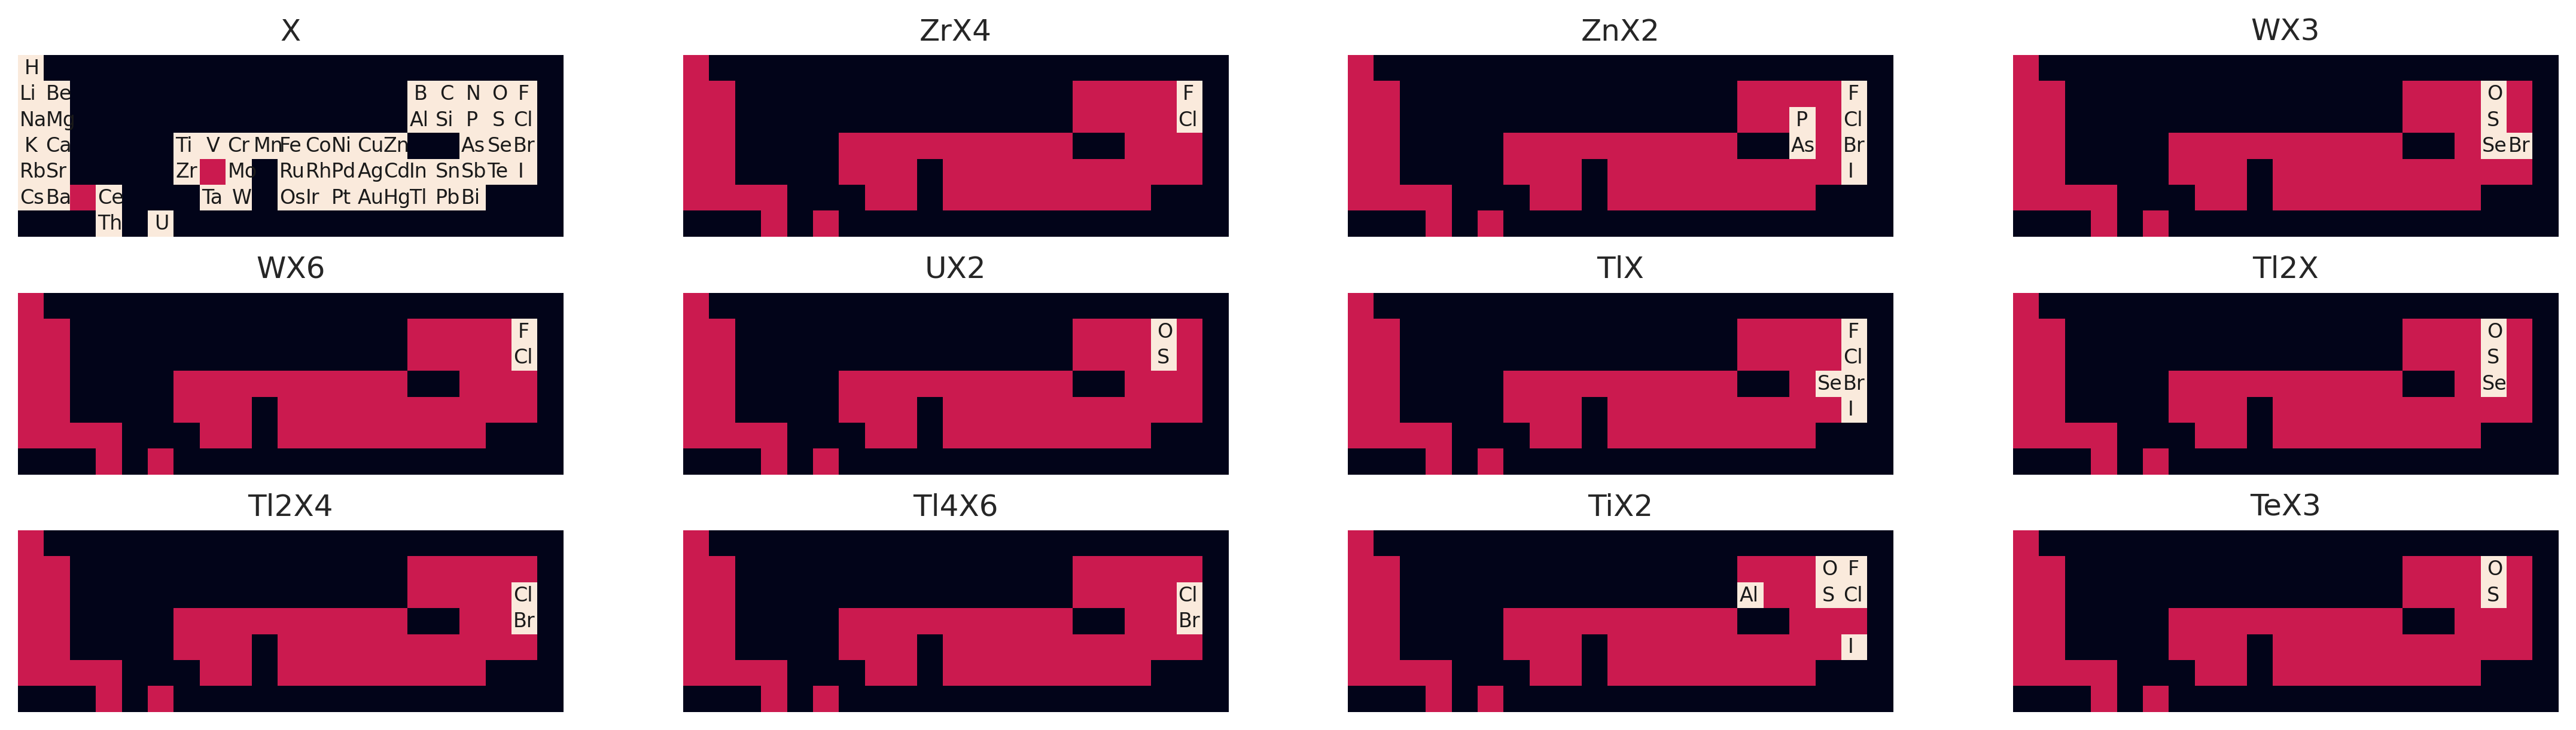
\includegraphics[width=18.0cm]{tables.png}
	\caption{Periodic table representation of the constructed dataset.}
	\label{fig:fig1}
\end{figure}

Here, black means no element exist at this position, red means an element in this position exists in dataset, and white means there exist a compound $R-X_n$ as explained above. In this example, for instance, the data shows that both $\ce{ZrF4}$ and $\ce{ZrCl4}$ exist in dataset, but there exist no other compound with formula $\ce{ZrX4}$. It also shows that most lanthanides and actinides, as well as Tc, Re, Ga and Ge hadn't been discovered to this date. The vertical relationships on this side of the PS are clear from this sample.

\section{Results and discussion}

\subsection{Mean Horizontal Neighbouring Distance}
From figure \ref{fig:fig1} the typical vertical similarity can be spoted in the majority of tables from this sample (manifested as vertical blocks of white squares). We may ask, however, to what extent is this vertical similarity rule followed throughout the whole dataset? That is, is it more prevalent than, for instance, horizontal or diagonal (or any other) similarity and, in any case, how much deviation is there from the ideal arrangement?

To answer this, the horizontal neighboring distance (HND) was computed. For each element in each table, this is calculated as the averaged difference in PS groups there exist from the element to all its neighbors in the same table. This quantity is then averaged throughout all tables and the result is shown in figure \ref{fig:fig2}. Note that this quantity is clearly a function of the available chemical space and the selected PS. By construction, an HND of 0 means the two elements belong in the same group, reinforcing the vertical similarity idea, while a larger distance implies a departure from this rule.

\begin{figure}[h!]
  \centering
	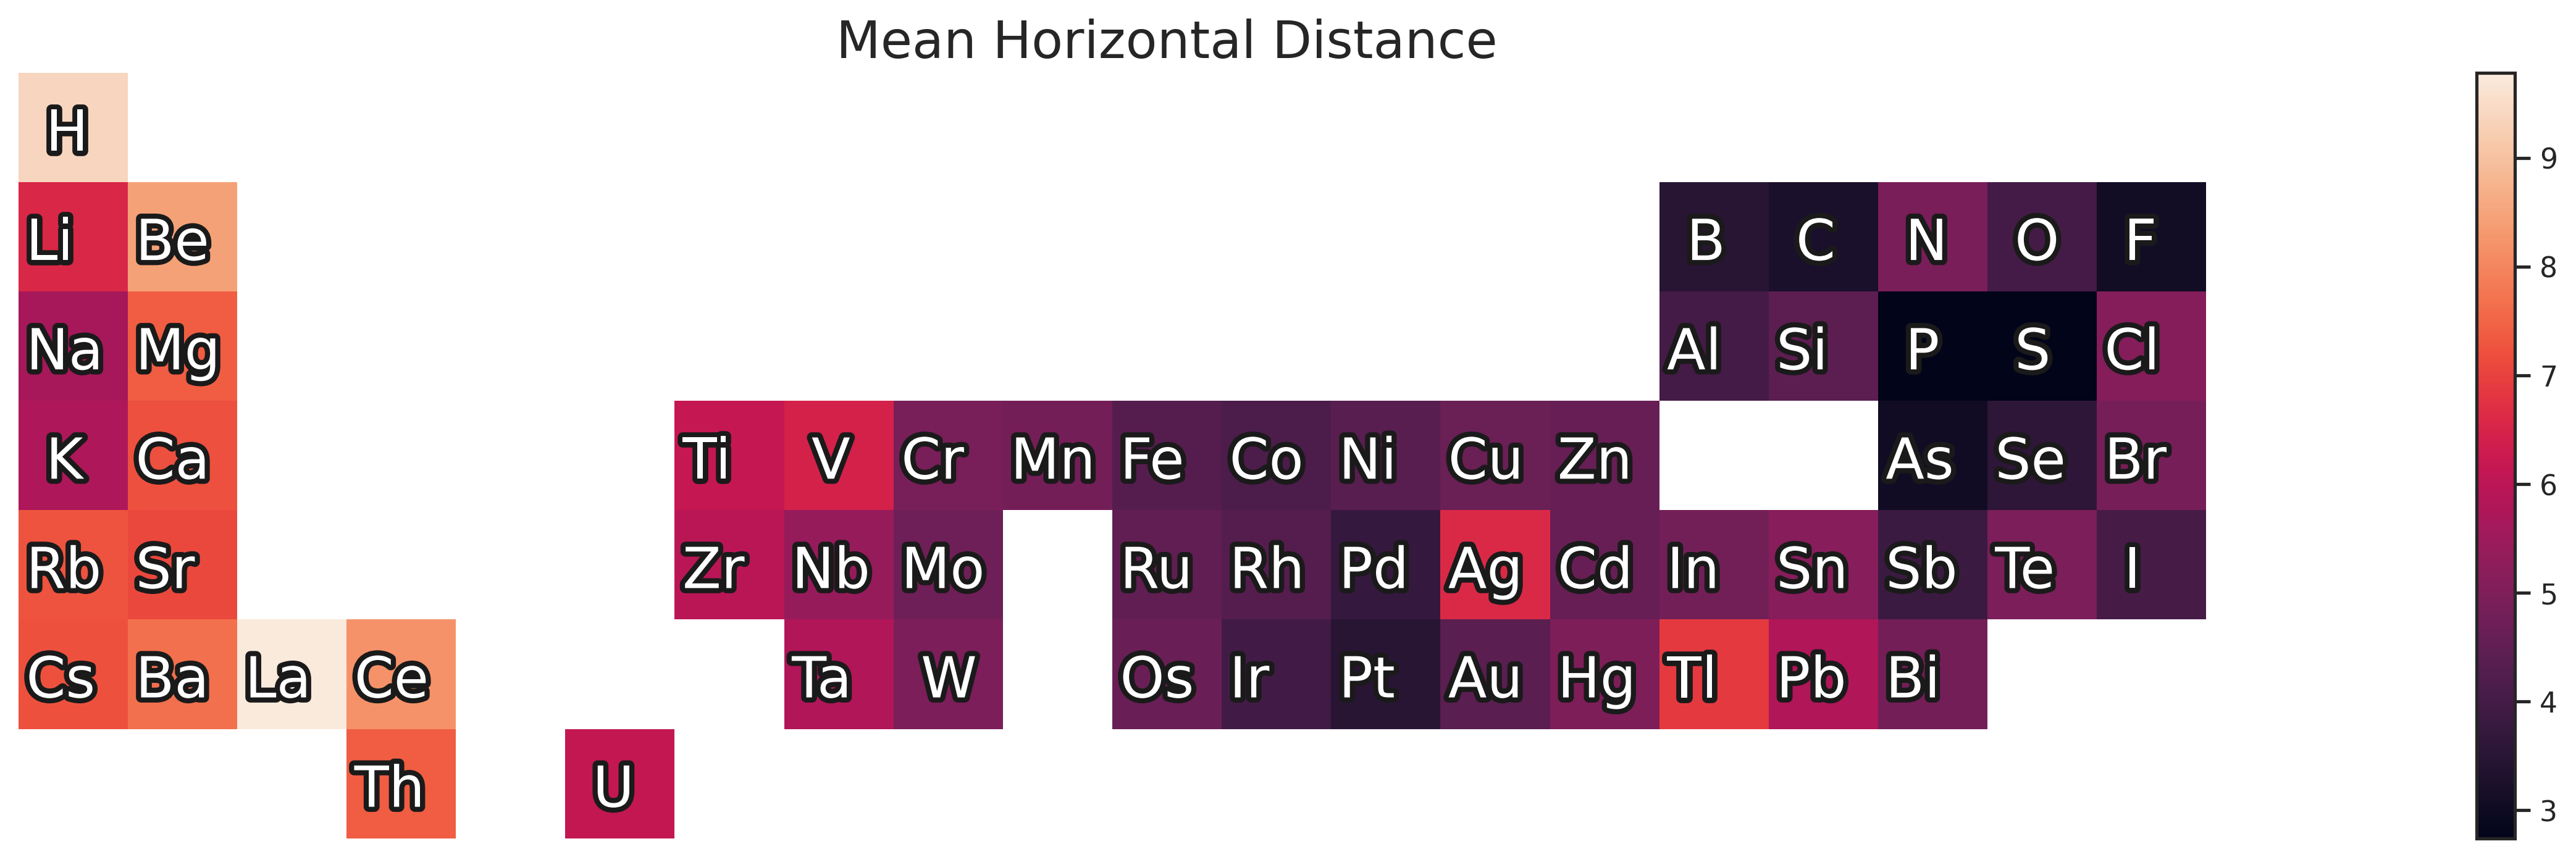
\includegraphics[width=16.0cm]{meanHND.png}
	\caption{Mean horizontal neighboring distance (HND) for the elements in the PS. HND measures up to what degree elements are "misslocated" in the PS considering that similarity should be expressed as vertical relationships. }
	\label{fig:fig2}
\end{figure}

Figure \ref{fig:fig2} clearly shows that, overall, the vertical similarities do not occur throughout the whole PS and, furthermore, this occurs more frequently to the right of the PT. Groups 1 and 2 show surprisingly high HNDs considering how chemically similar elements within these groups are expected to be (Na-K-Rb-Cs and Mg-Ca-Sr for instance). An initial explanation, for which more evidence will be shown further on, calls for the consideration of the metallic character of these elements which, in some aspects, resemble the chemistry of the transition metals (group 3-12) and thus are expected to appear in some of the tables, increasing the mean HND for the elements of these groups.

A number of other different distances can be calculated as well, but this has been selected as the most descriptive as the PS is constructed on the basis of order and similarity, with the similarity expresed as a strictly vertical one on this representation, as already stated above. Given that HND is parametrically a function of the selected PS, a new PS may now be devised by optimization of this quantity, which would lead to one where HND is minimized while preserving some given elemental ordering (be it atomic weight, Pettifor's scale, etc), which should naturally lead to a more expressive PS at least, and would allow a comparison between systems. Optimization and comparison between systems is, however, a topic for the next section.

\begin{figure}[h!]
  \centering
	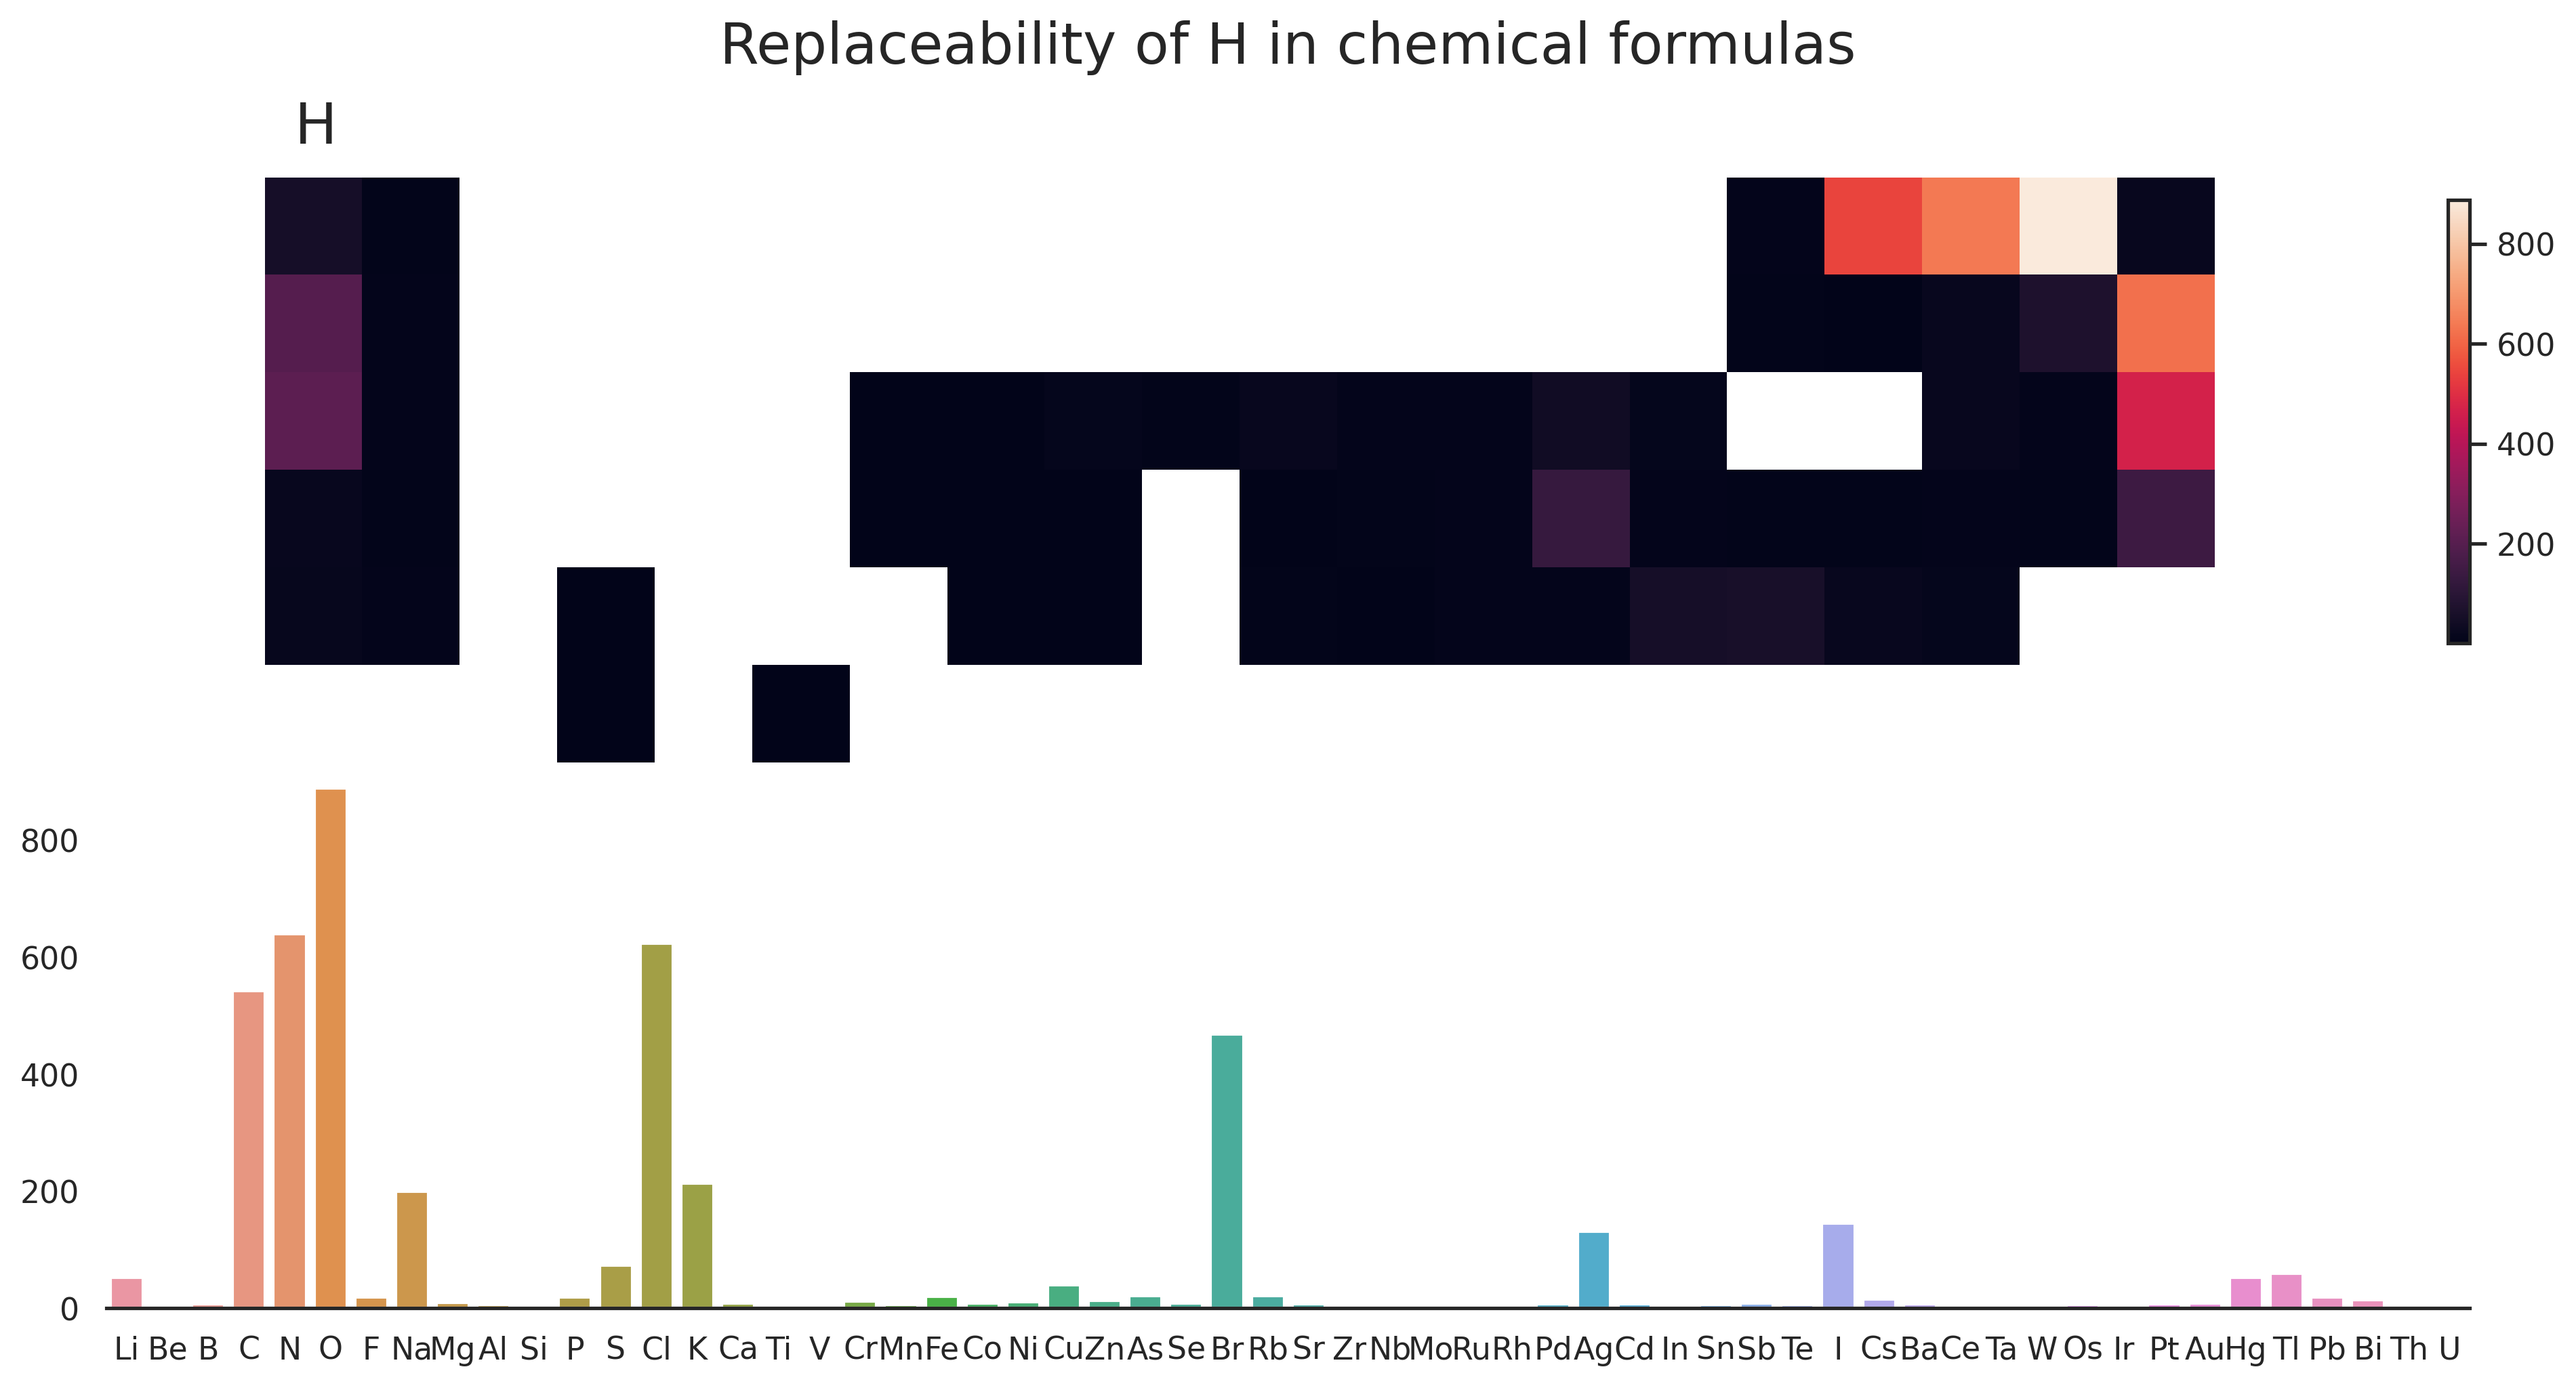
\includegraphics[width=13.0cm]{replace_H.png}
	\caption{Replaceability of H in compounds in dataset. a) PS format showing periodic relationships and b) Barplot showing elements in atomic number order, bar height is number of times H and this element appear in the same table.}
	\label{fig:fig3}
\end{figure}

\subsection{Replaceability of elements.}

Not only can we calculate how far away elements are from their neighbors, but we might as well ask who their neighbors are. From the way the data was preprocessed, the answer to latter question can be interpreted as a measure of replaceability, as elements in the same constructed set can be interchanged within this set's corresponding formula. For a given element, the calculation consists of taking all the tables that contain this element, and then for each other element count the number of times these are present in this subset of tables. From this, some more detailed insights can be obtained about the relationships between elements, as shown in figure \ref{fig:fig3} for hydrogen.

It can clearly be seen that H is, under our approximation, more similar to C, N and O, and the halogens (except F). A similarity with the halogens are expected, as in most of organic chemistry these appear as substituents of H, but the resultant similarities to C, N and O must be further explored in order for it to chemically make sense.

Although the relationship between O, C and N with H may seem weird, taking a look at the formulas responsible for this result it is found that $\ce{SX2}$, $\ce{OTlX}$, $\ce{NX3}$, $\ce{MoOX}$, $\ce{MnOX}$ and similar substances offer an explanation. These show that such a result is actually due to the presence of metallic oxides, hydroxides and hydrides, and happens in combination with elements with more than one oxidation state such as transition metals and other non-metals such as S and N, which allows them to combine in some compounds with a number $\textit{x}$ of Hs, while in other compounds with the same number of Os by doubling their oxidation state.

The other important relation found here is that expressed with the halogens. It can clearly be seen that the H-to-halogens relations are much stronger (more than twice) than that with the alkaline elements (group 1). This is clearly an important result as it suggests that H should be nearer to the halogens in the PS, as opposed to being in group 1 and treated as an alkaline element.

To show the power of these plots, another example is brought into play (figure \ref{fig:fig4}).

\begin{figure}[h!]
  \centering
	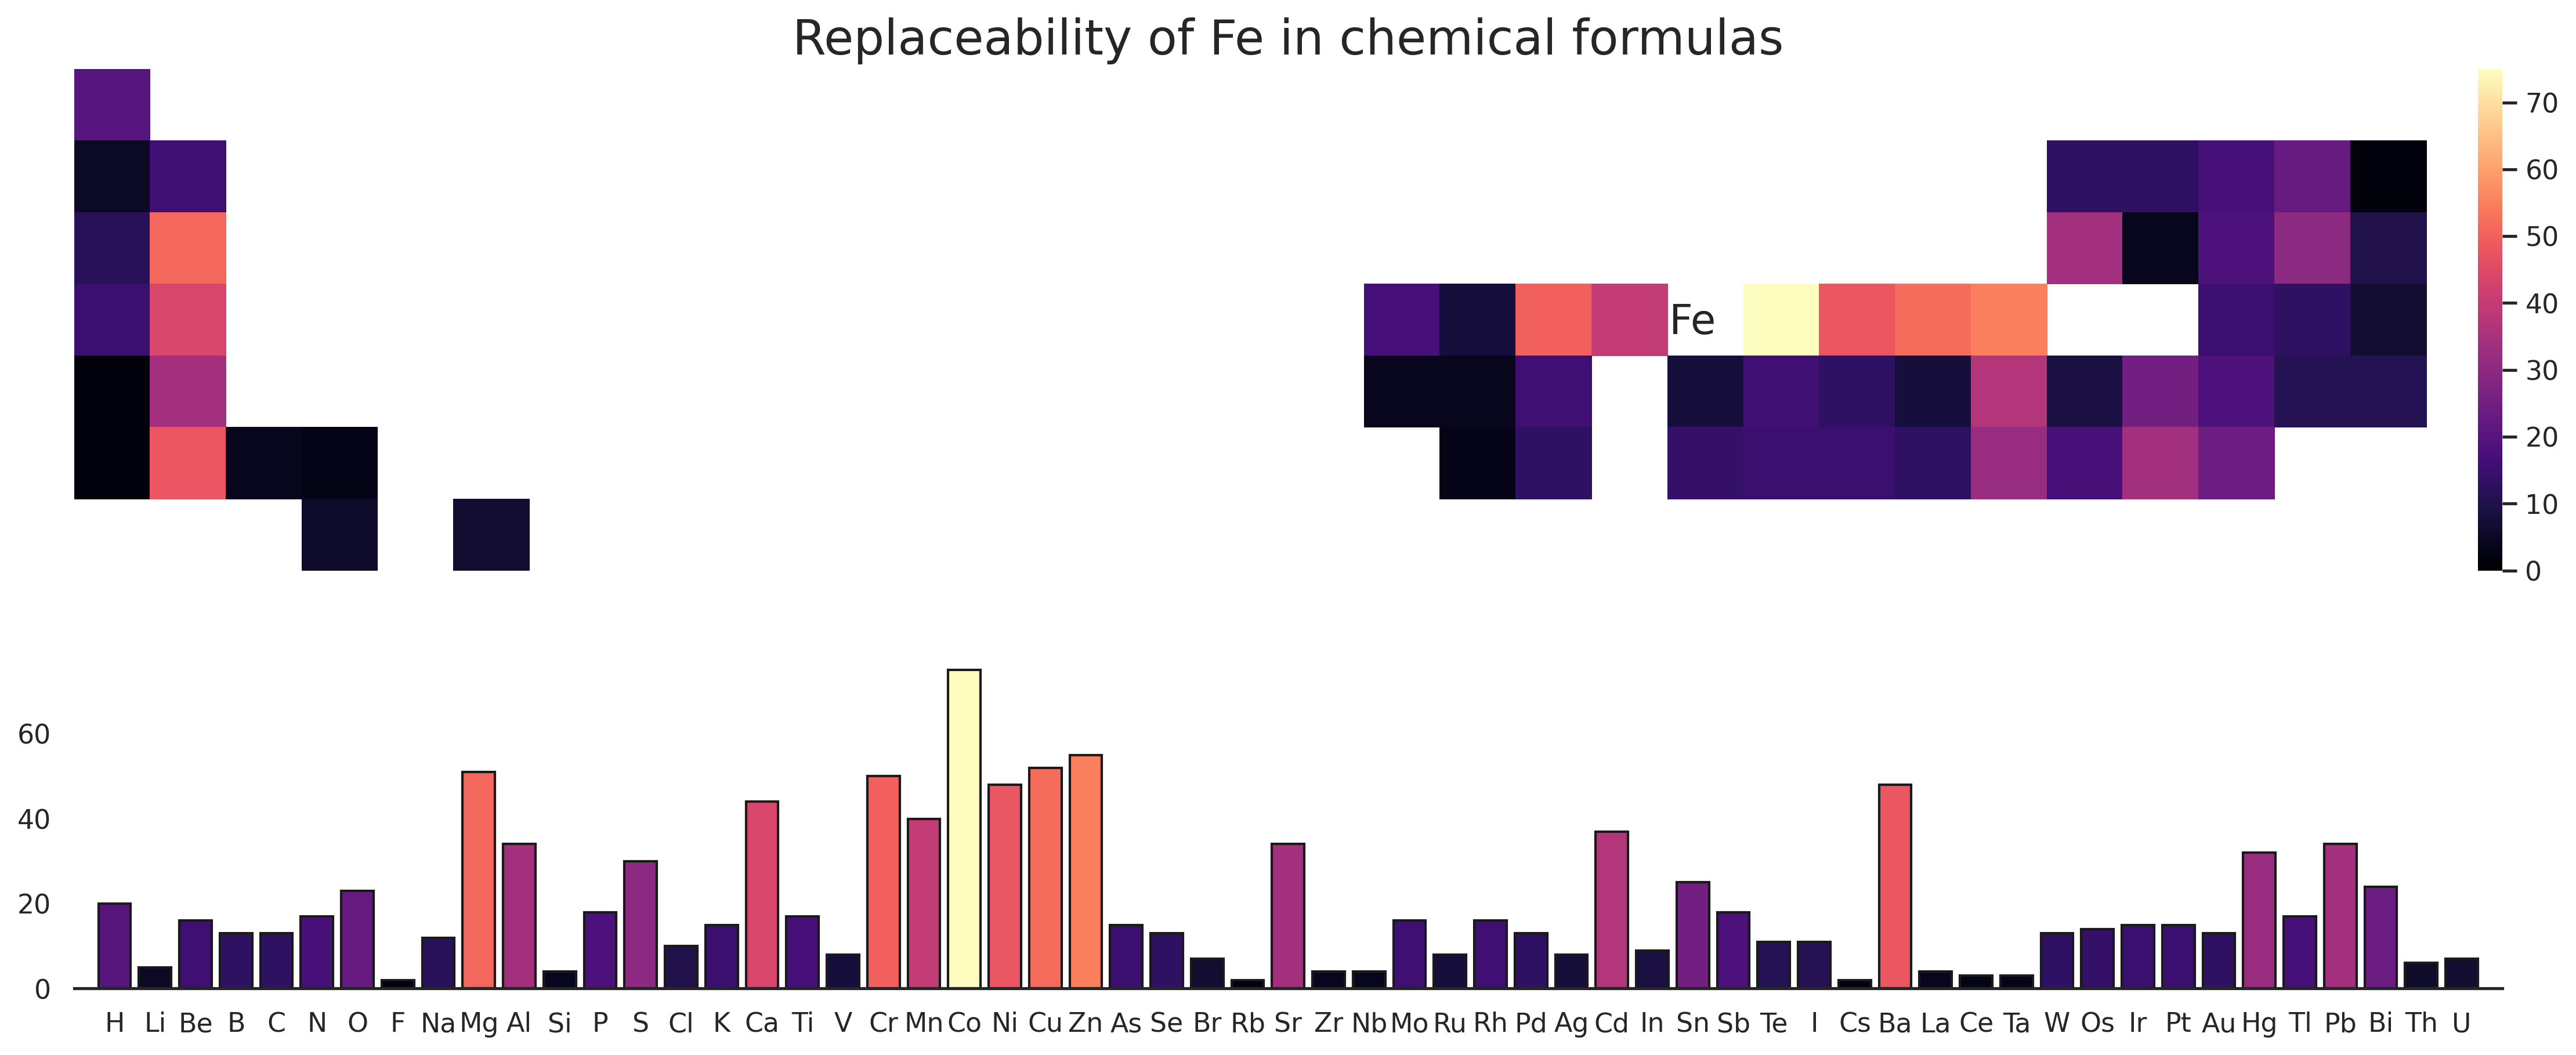
\includegraphics[width=13.0cm]{replace_Fe.png}
	\caption{Replaceability of Fe in compounds in dataset.}
	\label{fig:fig4}
\end{figure}

The replaceability plot for Fe shows that, for this element, the similarity is mostly horizontal along the 4th period transition metals, as already expressed by Mendeleev on his original publication of the PS, but it also shows a comparable similarity with alkaline earth elements (group 2). Such a similarity is a non-trivial result and deserves a more in-depth exploration, as the PS expresses none of this information in it. Some questions arise as, for instance, can a new PS be constructed, in such a way that this information is more explicitly given? If not, is there some particular reason (probably a topological one) for this?. As an additional observation, the plots for alkaline elements (Supplementary Information) do not show such a marked similarity to transition metals and are instead more cluttered around group 1 of PS.

One of these plots could be drawn for each element, but this becomes quite tedious as it would imply the production and analysis of more than 90 of these individually. Instead, the PS representations can be unravelled into a 1-dimensional format and normalized, and finally concatenated into one large square matrix so as to be able to visualize all pairwise relative similarities between elements, as shown in figure \ref{fig:fig5}. This ultimately looks much like a correlation matrix as it states element-wise relationships between pairs of elements in a more concise format. It looses, however, the possibility of studying the PS on the light of these results, showing that both representations give different important information and none should be disregarded in favor of the other. To facilitate the visualization of the first kind of representation (figures \ref{fig:fig3} and \ref{fig:fig4}) an interactive webpage is to be constructed, where the similarities are calculated for an user-chosen element and shown in the PS representation.
 
The details of the normalization are important as it determines what is shown on the figure and the way it should be interpreted. In this case each row of the matrix was divided by the maximum value of said row, which naturally corresponds to the same element as the row, justifying the observation that the diagonal of the matrix is all ones. Due to this normalization the matrix is not symmetric, meaning the information on the upper triangle is different than that shown on the lower triangle, which is the same as stating that the similarity relationship X $\rightarrow$ Y is not the same as Y $\rightarrow$ X. As an example, take the couple La-Fe. As can be seen, the row corresponding to La has a high value (near 1) at the Fe column, meaning La can be replaced by Fe most of the time (within this dataset). When we look at the Fe row, the value corresponding to La is one of the lowest, meaning Fe can not be replaced by La most of the time. 

The unidirectionality of these relationships is important as it may lead to several conclusions (drawn naively only from these results), namely:

\begin{itemize}
	\item The chemistry of La wasn't as explored as that of Fe at the time. This can be thought of in sociological terms, as an exploration of the new element (La) limited to trying to copy the chemistry of a seemingly similar element (Fe).
	\item Or possibly the chemistry of La is more restricted than that of Fe, meaning possibly that the oxidation numbers for La are only a subset of those for Fe.
\end{itemize}

\begin{figure}[h!]
  \centering
	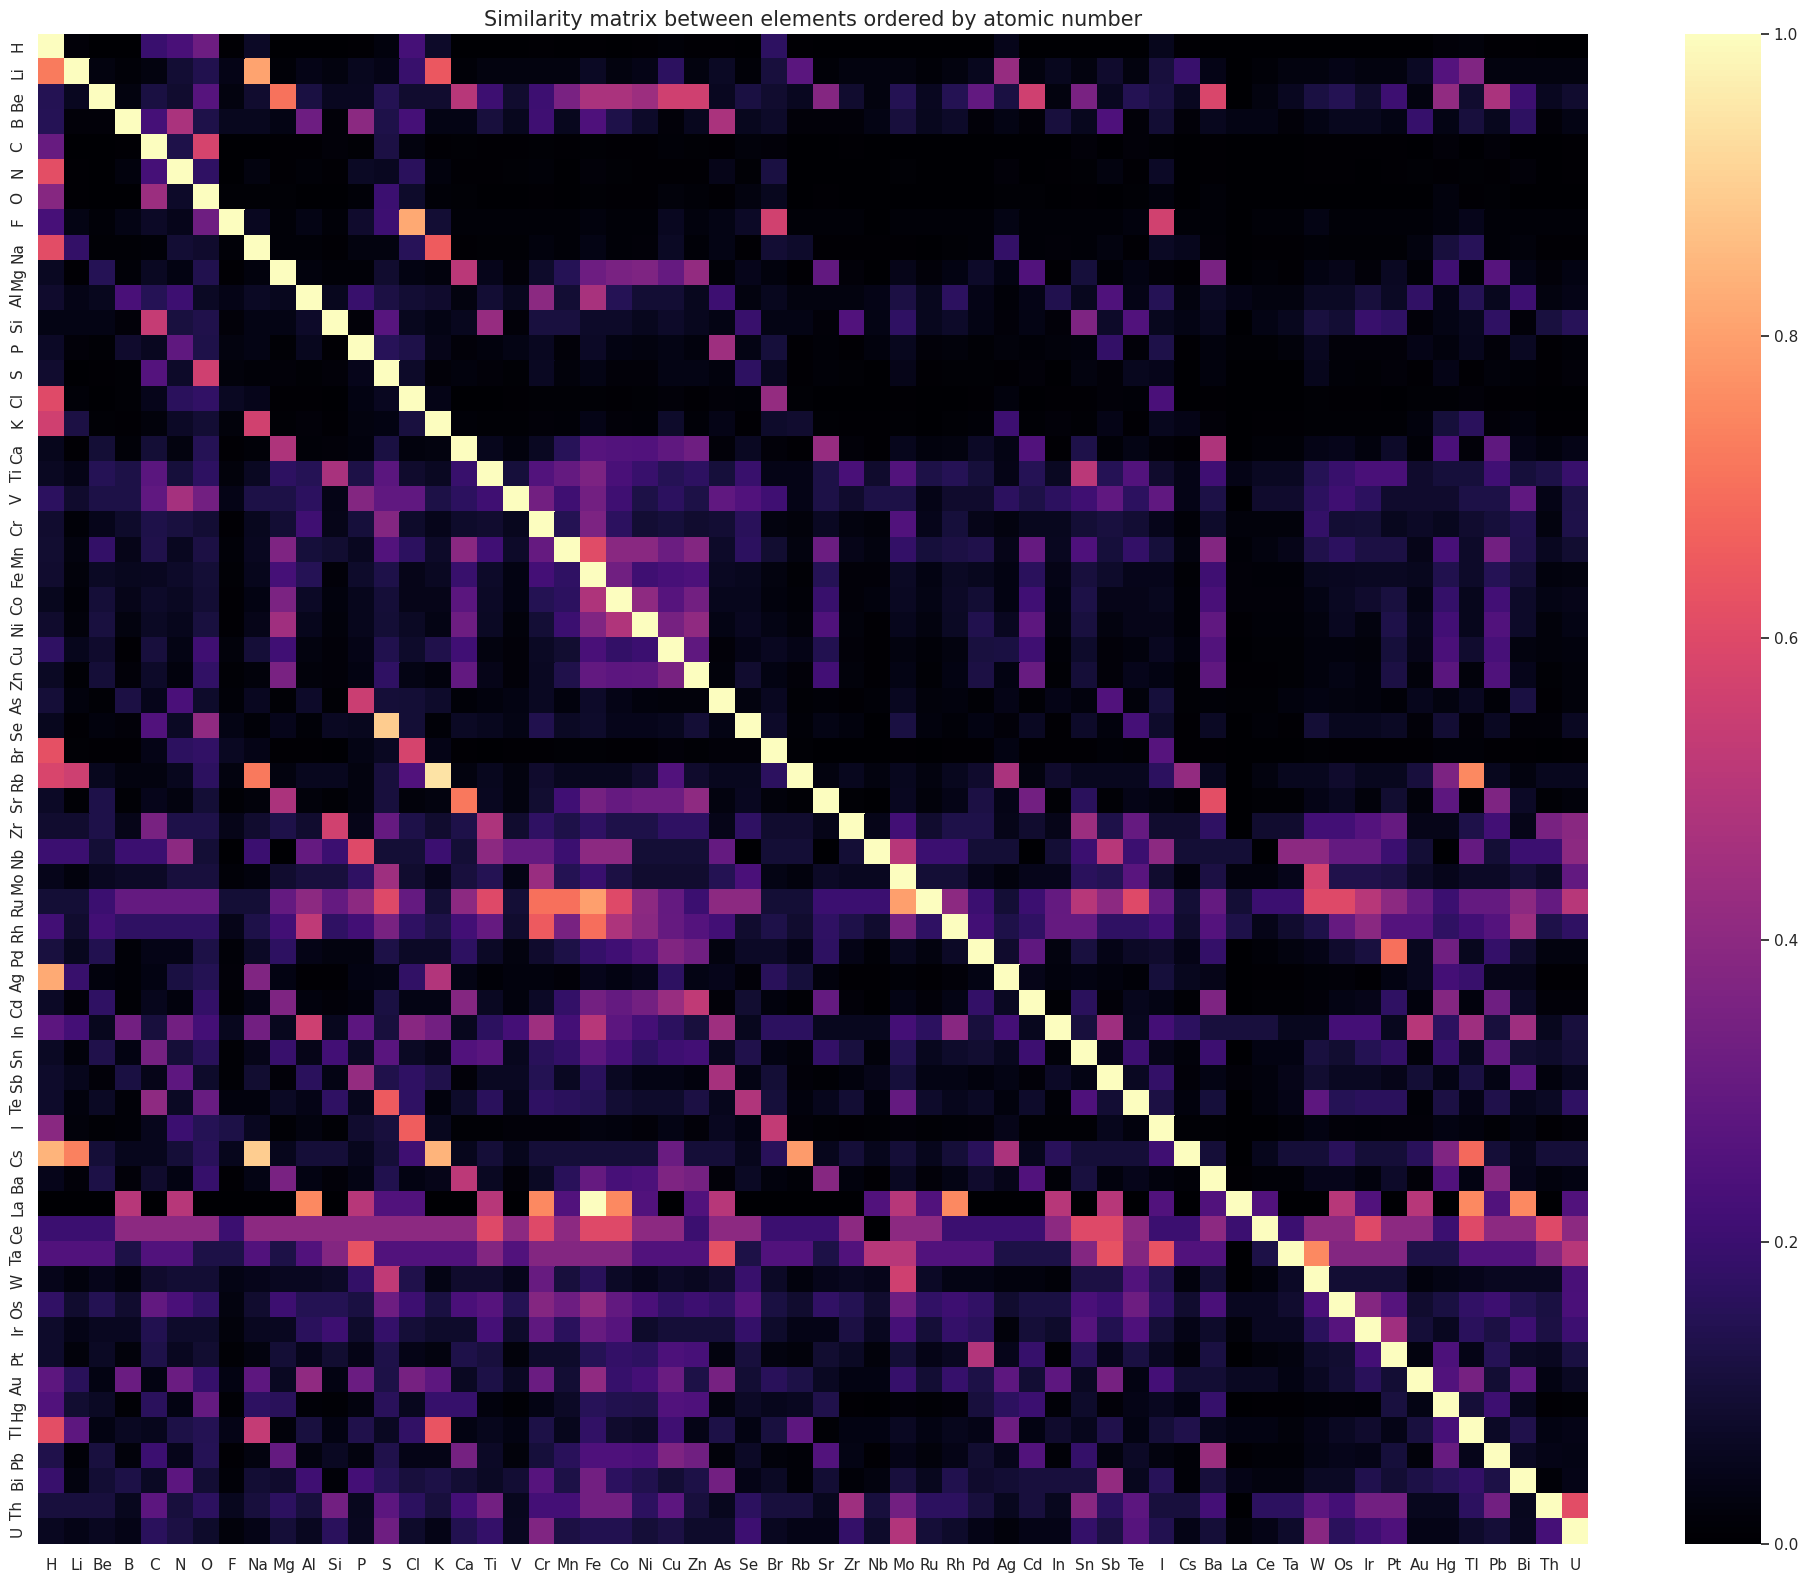
\includegraphics[width=18.0cm]{matrix.png}
	\caption{Replaceability matrix. Note that this matrix is not symmetric, meaning the relationship X $\rightarrow$ Y is not the same as Y $\rightarrow$ X.}
	\label{fig:fig5}
\end{figure}

In more general terms, some substructures can be seen within the matrix such as, for instance, vertical, horizontal and diagonal lines, which explicitly suggest the higher structure the PS is intended to capture. Namely, diagonal relationships on this matrix establish vertical pair-wise element similarities in the periodic table, for instance As $\rightarrow$ P followed by Se $\rightarrow$ S, Br $\rightarrow$ Cl, and so on. Vertical and horizontal relationships represent horizontal similarities in the PS, as well as other hidden ones such as the one shown in \ref{fig:fig4} between group 2 elements and first row transition metal elements. In this sense, this matrix (and others of this kind) allow for a much high level visualization of all the general relationships between elements without an embedding in any arbitrary PS. Again, some optimization work can be performed on this matrix similar to \cite{Glawe_2016}, where a reformulation of the Pettifor's scale was done with a similar approach to that presented here, but using only a set of inorganic substances obtained from the \href{https://ucsd.libguides.com/crystallography/icsd}{ICSD}. The present article could in fact be an extension of this, as it takes a very similar concept and extends it from inorganic solids to all known substances (up to some date).



\renewcommand\refname{References}
\bibliography{bib}
\bibliographystyle{ieeetr}

\end{document}             % End of document.

